% --- CÓDIGO ATUALIZADO para Analise/selection_sort_analise.tex ---

\subsubsection*{Análise de Complexidade e Teste de Mesa - Selection Sort}

\qquad Esta seção apresenta o teste de mesa do \textit{Selection Sort}, a derivação de sua função de tempo $T(n)$ e a análise de cada cenário.

\paragraph{Teste de Mesa}
\qquad A Figura \ref{fig:selection_mesa} mostra a execução do \textit{Selection Sort}, acompanhando o estado do vetor e das variáveis a cada passo do algoritmo na busca pelo menor elemento e seu posicionamento correto.

% --- IMAGEM DO TESTE DE MESA ---
\begin{figure}[htbp]
    \centering
    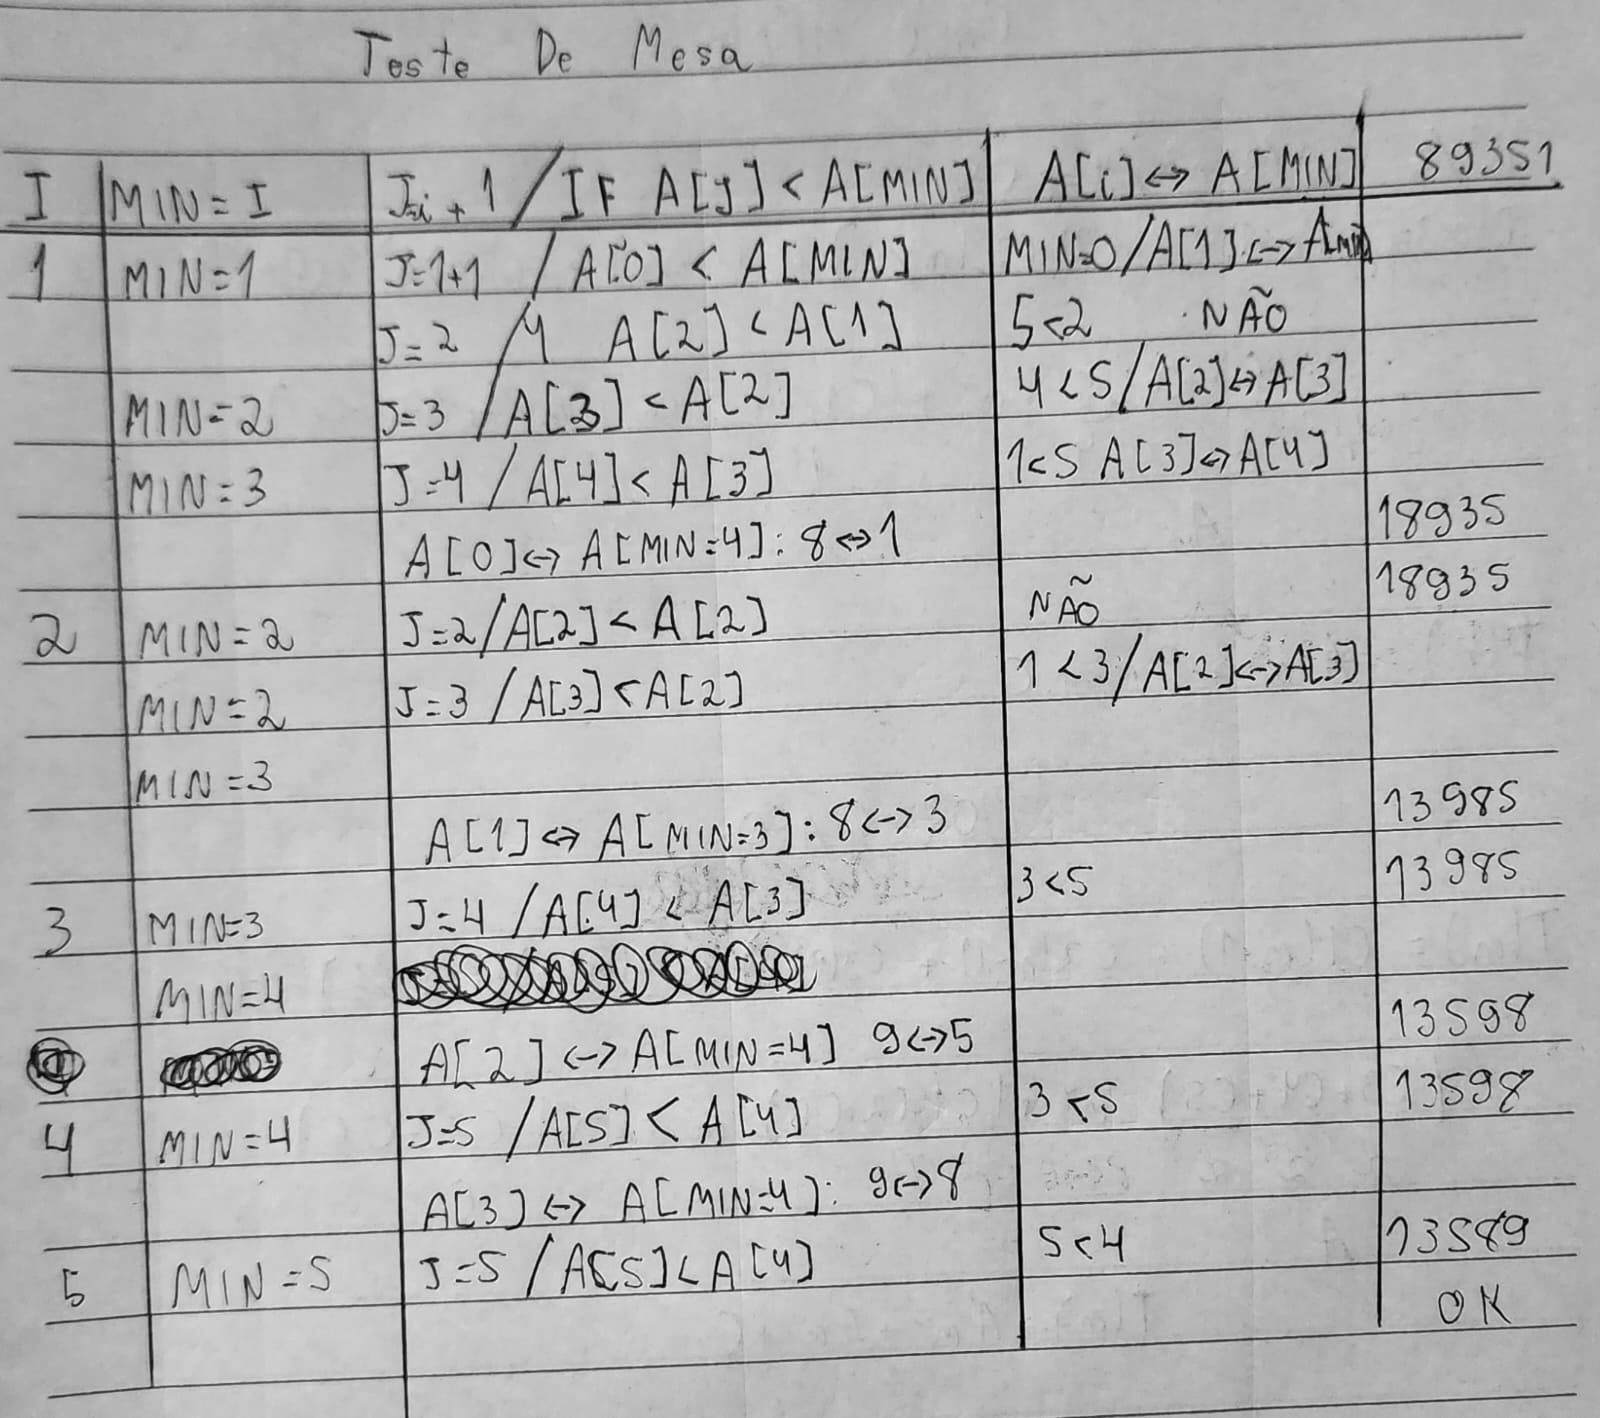
\includegraphics[width=1.0\textwidth]{Imagens/Selection Sort/testedemesa-selection.jpg}
    \caption{Teste de Mesa do algoritmo Selection Sort (elaborado pelo autor).}
    \label{fig:selection_mesa}
\end{figure}

\paragraph{Análise Matemática de Complexidade (Escrita)}
\qquad A função de tempo total, $T(n)$, é dada pela soma do custo de cada linha ($c_i$) multiplicado pelo número de vezes que ela é executada. Com base na tabela de custos apresentada na seção de Algoritmos, a equação geral é:
$$ T(n) = c_1(1) + c_2(n) + c_3(n-1) + c_4\left(\frac{n(n-1)}{2}\right) + c_5\left(\frac{n(n-1)}{2}\right) + c_6(\text{soma}) + c_7(n-1) $$
\qquad Agrupando os termos por potência de $n$, o termo dominante é proporcional a $n^2$, originado pelos laços aninhados:
$$ T(n) = \left(\frac{c_4+c_5}{2}\right)n^2 + \dots $$
\qquad Assim, a função de tempo do \textit{Selection Sort} é sempre quadrática, na forma $An^2 + Bn + C$. A única variação entre os cenários está no valor da "soma" (custo $c_6$, referente às atualizações de \texttt{min\_idx}), que não influencia o termo dominante. Por isso, a complexidade é $O(n^2)$ em todos os casos.


\paragraph{Análise por Cenário (com Imagens)}
\qquad A seguir, o resultado dessa análise é detalhado para cada cenário.

\qquad No \textbf{melhor caso} (Figura \ref{fig:selection_melhor_math}), mesmo com o vetor já ordenado, a complexidade permanece $O(n^2)$, já que todas as comparações são realizadas independentemente da ordem inicial dos elementos.

% --- IMAGEM DO MELHOR CASO ---
\begin{figure}[htbp]
    \centering
    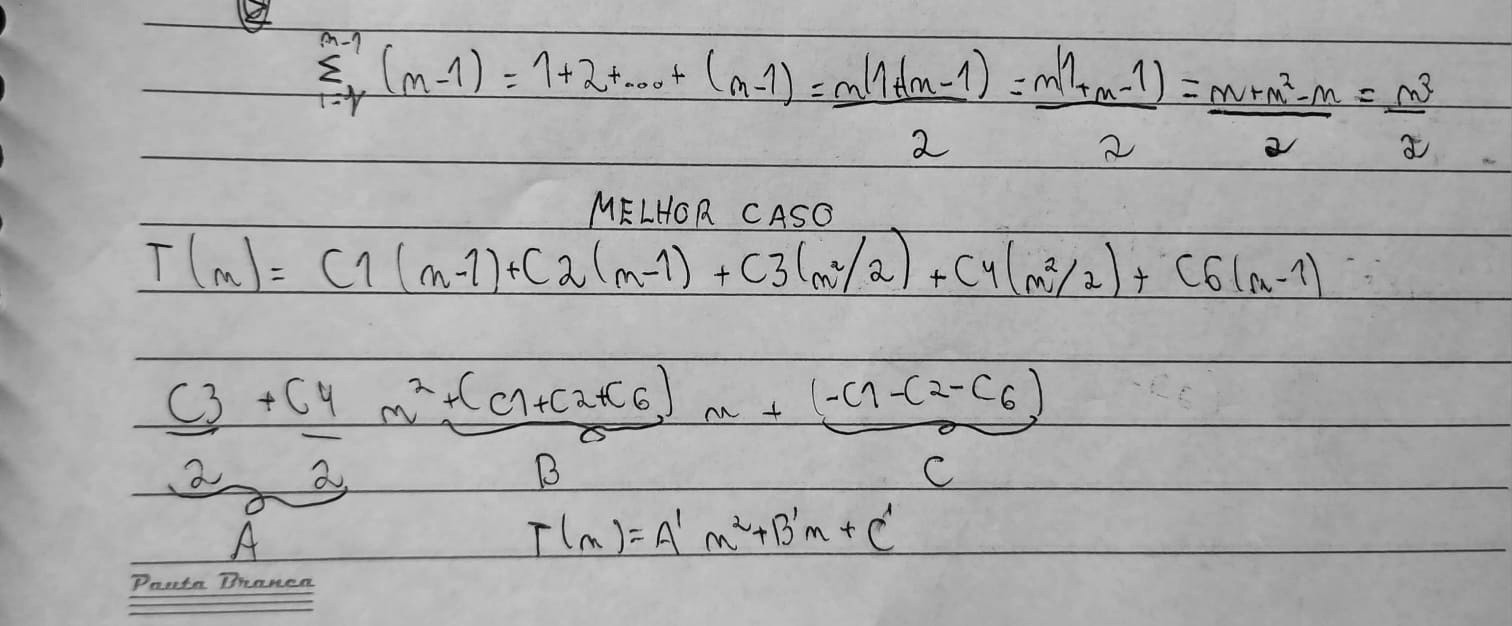
\includegraphics[width=0.9\textwidth]{Imagens/Selection Sort/melhorcaso-selection.jpg}
    \caption{Análise manuscrita para o Melhor Caso do Selection Sort (elaborado pelo autor).}
    \label{fig:selection_melhor_math}
\end{figure}

\qquad No \textbf{pior caso} (Figura \ref{fig:selection_pior_math}), com o vetor em ordem inversa, o número de comparações não se altera, mantendo a mesma complexidade $O(n^2)$.

% --- IMAGEM DO PIOR CASO ---
\begin{figure}[htbp]
    \centering
    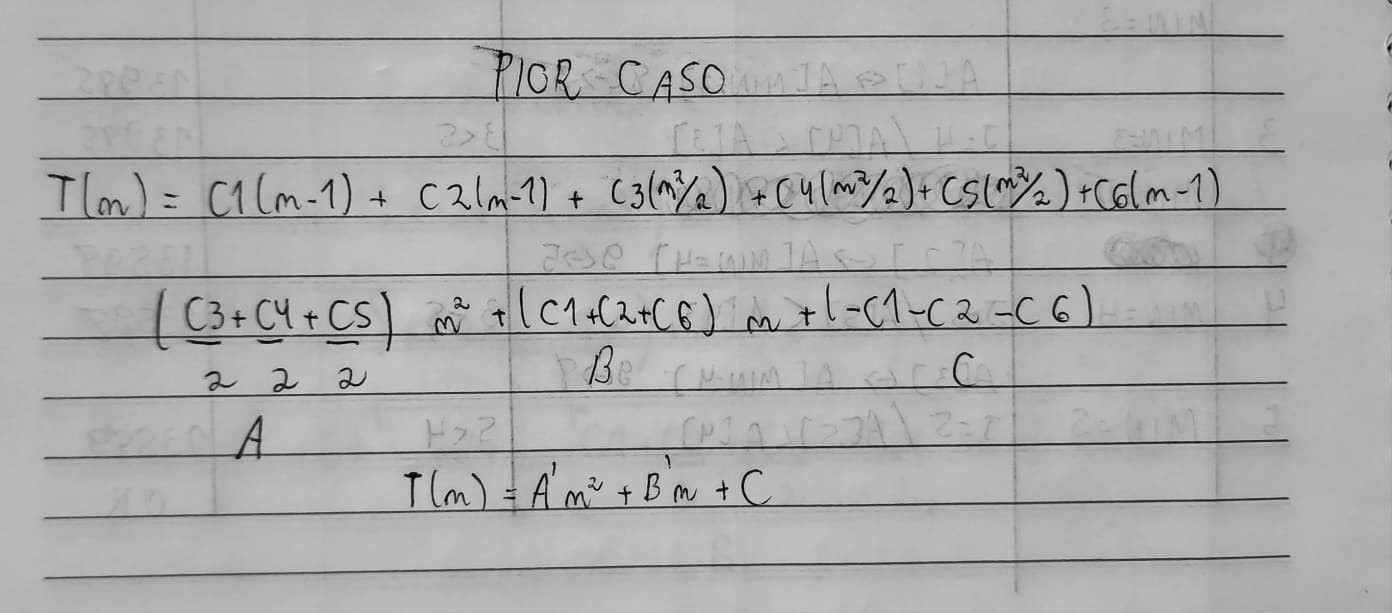
\includegraphics[width=0.9\textwidth]{Imagens/Selection Sort/piorcaso-selection.jpg}
    \caption{Análise manuscrita para o Pior Caso do Selection Sort (elaborado pelo autor).}
    \label{fig:selection_pior_math}
\end{figure}

\qquad No \textbf{caso médio} (Figura \ref{fig:selection_medio_math}), o resultado é o mesmo, com complexidade $O(n^2)$.

% --- IMAGEM DO CASO MÉDIO ---
\begin{figure}[htbp]
    \centering
    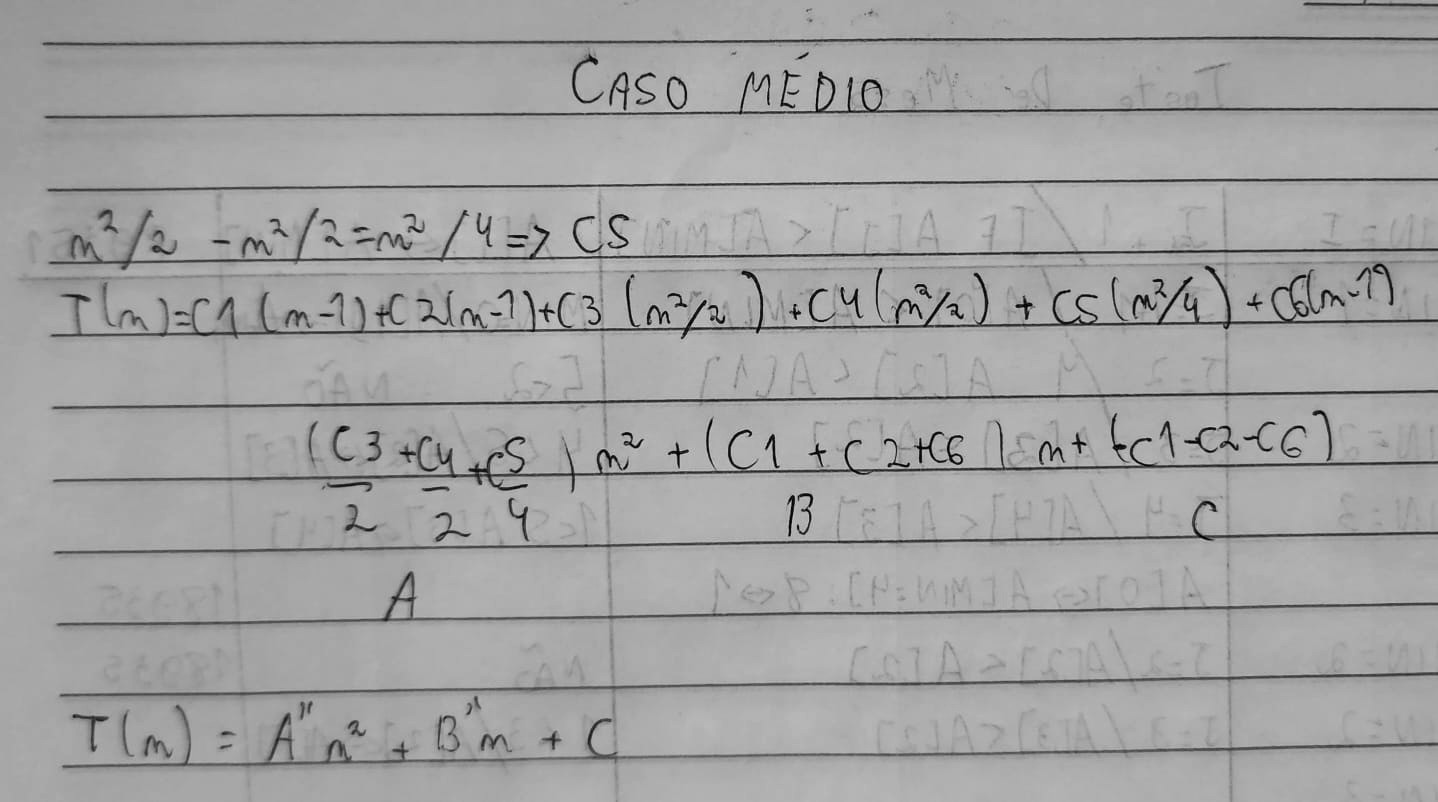
\includegraphics[width=0.9\textwidth]{Imagens/Selection Sort/mediocaso-selection.jpg}
    \caption{Análise manuscrita para o Caso Médio do Selection Sort (elaborado pelo autor).}
    \label{fig:selection_medio_math}
\end{figure}

\FloatBarrier

\qquad Quanto à \textbf{complexidade de espaço}, o \textit{Selection Sort} apresenta complexidade $O(1)$, pois a ordenação é feita \textit{in-place}, sem uso de estruturas auxiliares proporcionais a $n$.